This section describes the performance achieved by the model when predicting the number of threads and core composition to use for each of the StreamIt benchmarks and compares it to the optimal solution found when exploring the space.

\begin{figure}[t]
    \centering
    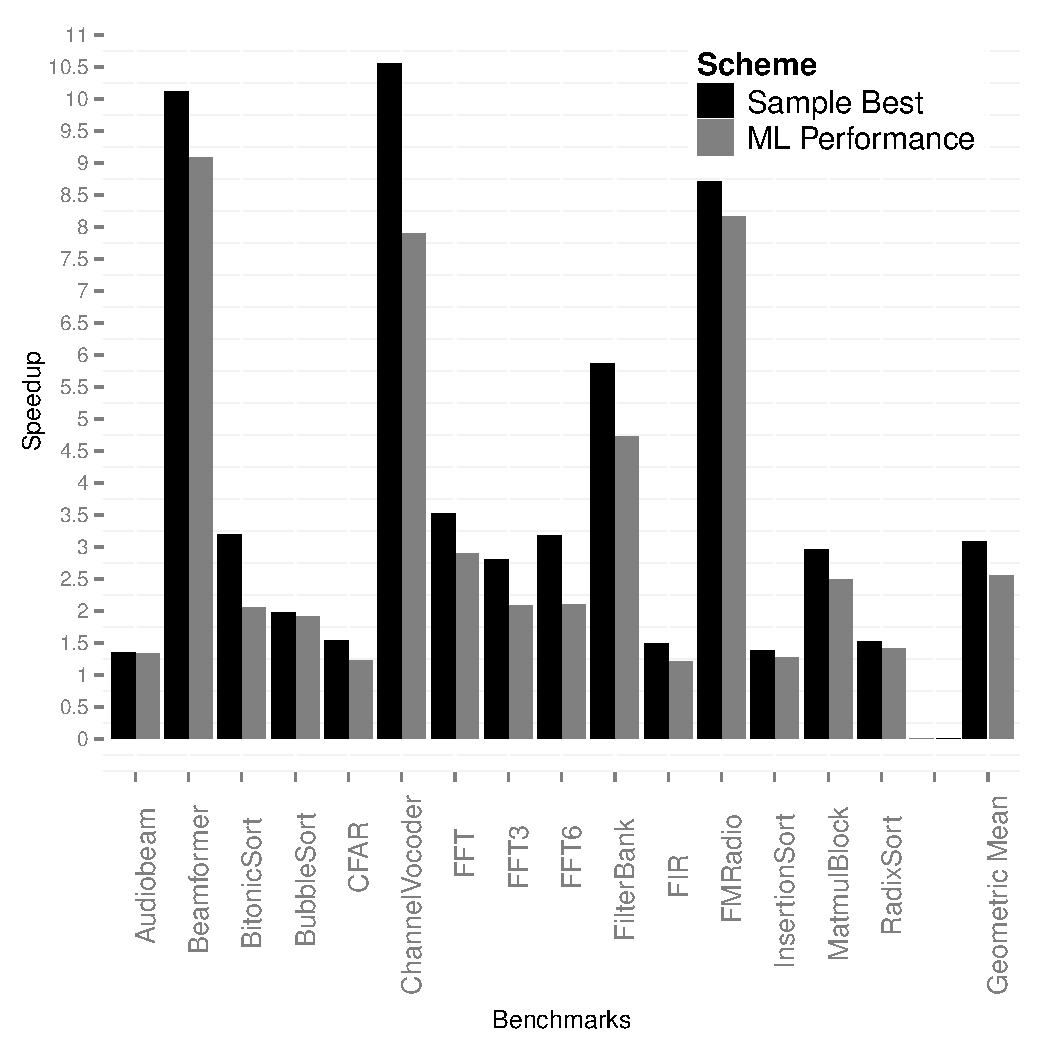
\includegraphics[width=0.7\textwidth]{streamit-paper/graphics/results.pdf}
    \caption{Performance of the machine-learning model against the best execution from random sampling. The baseline for the speedup measurement is single core, single-working-thread execution using O2 compiler optimisations. Higher is better.}\label{fig:results}
\end{figure}

\subsection{Machine Learning Model Evaluation Methodology}

Leave-one-out cross-validation defined in Chapter~\ref{chp:Background} Section~\ref{sec:valid} is used for testing the linear model.
This is standard methodology in the machine-learning community ensuring that the training data is never used for testing.
For the kNN model, the training data consists of all the generated synthetic benchmarks and it is only tested on the real StreamIt applications as they are not used for training.
To obtain the speedup the performance of the machine learning based result are compared to the best from the sample space to running the StreamIt benchmark on a single core, single-working-thread, using O2 compiler optimisations. 

\subsection{Evaluation}

Figure~\ref{fig:results} compares the performance of the machine-learning model and the best performance from the sample space.
As explained in the earlier section, the sampled best is drawn from a sample size of 1,316 combinations of core compositions and thread partitions for each application when possible.
The baseline is the original StreamIt application running with one thread and one core with O2 optimisations on the dynamic multi-core processor.
The average speedup obtained through the machine-learning model is 2.6x compared to the baseline, this is only 16\% smaller than the average of the best found, which is a speedup of 3.1x.
These results are positive as it means the model's results are at least within 16\% of the total best.

As can been seen in Figure~\ref{fig:results} the largest performance penalty resides in the performance of \bench{ChannelVocoder}.
Table~\ref{tab:summary} presents the actual configuration found for the best sampled point and the machine-learning model prediction.
Each column represents a different thread and the number in the cell represents the number of cores associated with that thread.
For ~\bench{ChannelVocoder} the model predicts only 8 threads rather than the optimal 13.
Referring back to Figure~\ref{fig:threadtrend} and Figure~\ref{fig:overviewhist} from Section~\ref{sec:streamit:dse} \bench{ChannelVocoder} always performs better when adding more threads rather than increasing the size of a core composition.
This is the cause of the performance penalty, for ~\bench{ChannelVocoder} it is more important to allocate a higher number of threads rather than compose cores.
Aside from this case, the machine-learning model obtains similar speedups to the best sample.

For other applications such as ~\bench{Beamformer} and ~\bench{FMRadio}, the model is able to get very close to the optimal performance.
Both benchmarks obtain at least an 8x speedup when using the model.
This is an encouraging result as it shows that static-ahead of time partitioning of a DMP is an effective way of getting a good configuration.
In fact, the difference of configurations for ~\bench{FMRadio} between the best point from the space and the machine-learning model's is only of two cores which is small.

\begin{table*}[t]
\centering
\resizebox{0.75\textwidth}{!}{\begin{minipage}{0.5\textwidth}
  \small
  \hspace{-5em}
 \begin{tabular} { | l | l | l | l | l | l | l | l | l | l |l| }
    \hline
      & \textbf{1} & \textbf{2} & \textbf{3} & \textbf{4} & \textbf{5} & \textbf{6} & \textbf{7} & \textbf{8} & \textbf{9} & \textbf{10} \\ \hline
    B Audiobeam & 3 & 2 & \cellcolor[gray]{0.3}& \cellcolor[gray]{0.3}& \cellcolor[gray]{0.3}& \cellcolor[gray]{0.3}& \cellcolor[gray]{0.3}& \cellcolor[gray]{0.3}& \cellcolor[gray]{0.3}& \cellcolor[gray]{0.3} \\ \hline 
    M Audiobeam & 2 & 3 & \cellcolor[gray]{0.3}& \cellcolor[gray]{0.3}& \cellcolor[gray]{0.3} & \cellcolor[gray]{0.3}& \cellcolor[gray]{0.3}& \cellcolor[gray]{0.3}& \cellcolor[gray]{0.3}& \cellcolor[gray]{0.3}\\ \hline\hline
    B Beamformer & 1 & 4 & 2 & 4 & 4& \cellcolor[gray]{0.3}& \cellcolor[gray]{0.3}& \cellcolor[gray]{0.3}& \cellcolor[gray]{0.3}& \cellcolor[gray]{0.3} \\ \hline 
    M Beamformer & 6 & 4 & 4& \cellcolor[gray]{0.3}& \cellcolor[gray]{0.3}& \cellcolor[gray]{0.3}& \cellcolor[gray]{0.3}& \cellcolor[gray]{0.3}& \cellcolor[gray]{0.3}& \cellcolor[gray]{0.3} \\ \hline\hline
    B BitonicSort & 3 & 2 & 2 & 2 & \cellcolor[gray]{0.3}& \cellcolor[gray]{0.3}& \cellcolor[gray]{0.3}& \cellcolor[gray]{0.3}& \cellcolor[gray]{0.3}& \cellcolor[gray]{0.3}  \\ \hline
    M BitonicSort & 1 & 2 & 2 & 1 & 2 & 2 & 2 & \cellcolor[gray]{0.3}& \cellcolor[gray]{0.3}& \cellcolor[gray]{0.3} \\ \hline\hline
    B BubbleSort & 3 & 3& \cellcolor[gray]{0.3} & \cellcolor[gray]{0.3} & \cellcolor[gray]{0.3}& \cellcolor[gray]{0.3}& \cellcolor[gray]{0.3}& \cellcolor[gray]{0.3}& \cellcolor[gray]{0.3}& \cellcolor[gray]{0.3} \\ \hline
    M BubbleSort & 2 & \cellcolor[gray]{0.3} & \cellcolor[gray]{0.3} & \cellcolor[gray]{0.3} & \cellcolor[gray]{0.3}& \cellcolor[gray]{0.3}& \cellcolor[gray]{0.3}& \cellcolor[gray]{0.3}& \cellcolor[gray]{0.3}& \cellcolor[gray]{0.3} \\ \hline\hline
    B CFAR & 3 & 2 & \cellcolor[gray]{0.3} & \cellcolor[gray]{0.3} & \cellcolor[gray]{0.3}& \cellcolor[gray]{0.3}& \cellcolor[gray]{0.3}& \cellcolor[gray]{0.3}& \cellcolor[gray]{0.3}& \cellcolor[gray]{0.3} \\ \hline 
    M CFAR & 2 & 2  & 1  & 2 & \cellcolor[gray]{0.3}& \cellcolor[gray]{0.3}& \cellcolor[gray]{0.3}& \cellcolor[gray]{0.3}& \cellcolor[gray]{0.3}& \cellcolor[gray]{0.3} \\ \hline\hline
    B ChannelVoc.& 4 & 1 & 1 & 1 & 1 & 1 & 2 & 1 & 1 & 1 \\ \hline 
    M ChannelVoc.& 2 & 2 & 1 & 2 & 2& 2 & 2& \cellcolor[gray]{0.3}& \cellcolor[gray]{0.3}& \cellcolor[gray]{0.3} \\ \hline\hline
    B FIR & 3 & 2 &\cellcolor[gray]{0.3}&\cellcolor[gray]{0.3}&\cellcolor[gray]{0.3}&\cellcolor[gray]{0.3}&\cellcolor[gray]{0.3}&\cellcolor[gray]{0.3}&\cellcolor[gray]{0.3}&\cellcolor[gray]{0.3}\\ \hline
    M FIR & 2 & 2&\cellcolor[gray]{0.3}&\cellcolor[gray]{0.3}&\cellcolor[gray]{0.3}&\cellcolor[gray]{0.3}&\cellcolor[gray]{0.3}&\cellcolor[gray]{0.3}&\cellcolor[gray]{0.3}&\cellcolor[gray]{0.3}\\ \hline\hline
    \end{tabular}
  \end{minipage}	\hfill
  \hspace{1em}
\begin{minipage}{0.5\textwidth}

	 \begin{tabular} { | l | l | l | l | l | l | l |}
    \hline
      & \textbf{1} & \textbf{2} & \textbf{3} & \textbf{4} & \textbf{5} & \textbf{6}  \\ \hline

	B FFT & 3 & 3 & 5 & \cellcolor[gray]{0.3}& \cellcolor[gray]{0.3}& \cellcolor[gray]{0.3} \\ \hline
    M FFT & 6& 5 & 2& \cellcolor[gray]{0.3}& \cellcolor[gray]{0.3}& \cellcolor[gray]{0.3}  \\ \hline\hline
    B FFT3 & 3 & 2 & 2& \cellcolor[gray]{0.3}& \cellcolor[gray]{0.3}& \cellcolor[gray]{0.3} \\ \hline 
    M FFT3 & 3 & 2 & 3 & 3& 3& 3 \\ \hline\hline
    B FFT6 & 7 & 8& \cellcolor[gray]{0.3}& \cellcolor[gray]{0.3}& \cellcolor[gray]{0.3}& \cellcolor[gray]{0.3}\\ \hline
    M FFT6& 14 & \cellcolor[gray]{0.3}& \cellcolor[gray]{0.3}& \cellcolor[gray]{0.3}& \cellcolor[gray]{0.3}& \cellcolor[gray]{0.3} \\ \hline\hline
    B FilterBank & 4 & 5 & 6& \cellcolor[gray]{0.3}& \cellcolor[gray]{0.3}& \cellcolor[gray]{0.3} \\ \hline
    M FilterBank & 4 & 5 & \cellcolor[gray]{0.3} & \cellcolor[gray]{0.3}& \cellcolor[gray]{0.3}& \cellcolor[gray]{0.3}\\ \hline\hline
    B FMRadio & 7 & 6 & \cellcolor[gray]{0.3}& \cellcolor[gray]{0.3}& \cellcolor[gray]{0.3}& \cellcolor[gray]{0.3}\\ \hline
    M FMRadio & 7 & 4 & \cellcolor[gray]{0.3} & \cellcolor[gray]{0.3}& \cellcolor[gray]{0.3}& \cellcolor[gray]{0.3} \\ \hline\hline
    B InsertionSort & 3 & 2& \cellcolor[gray]{0.3}& \cellcolor[gray]{0.3}& \cellcolor[gray]{0.3}& \cellcolor[gray]{0.3} \\ \hline
    M InsertionSort & 3 & \cellcolor[gray]{0.3}& \cellcolor[gray]{0.3}& \cellcolor[gray]{0.3}& \cellcolor[gray]{0.3}& \cellcolor[gray]{0.3}\\ \hline\hline
    B MatmulBlock & 3 & 4 & 6 & 2 & \cellcolor[gray]{0.3} & \cellcolor[gray]{0.3}\\ \hline
    M MatmulBlock & 4 & 4 & \cellcolor[gray]{0.3}& \cellcolor[gray]{0.3}& \cellcolor[gray]{0.3}& \cellcolor[gray]{0.3}\\ \hline\hline
    B RadixSort & 3 & 3& \cellcolor[gray]{0.3}& \cellcolor[gray]{0.3}& \cellcolor[gray]{0.3}& \cellcolor[gray]{0.3}\\ \hline
    M RadixSort & 2 & 2& \cellcolor[gray]{0.3}& \cellcolor[gray]{0.3}& \cellcolor[gray]{0.3}& \cellcolor[gray]{0.3}\\ \hline
    
 \end{tabular}
  \end{minipage}}
  \caption{Number of Threads and Cores used for Best of Sample Space and Machine Learning Model.}\label{tab:summary}

\end{table*}

 \subsection{Summary}

This section has shown that it is possible to build a machine-learning model that achieves high level of performance using source code features.
In many applications, the model comes very close to the best from the sampled space, showing that the features used contain enough information to inform the model about the best decision.
